\documentclass[]{standalone}
\usepackage{commands}

\begin{document}
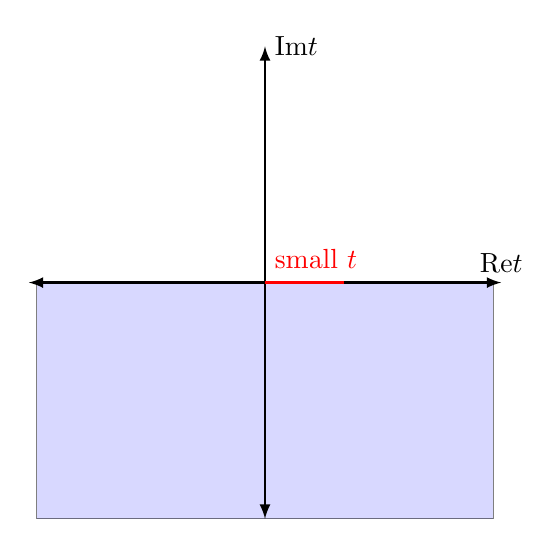
\begin{tikzpicture}
    \draw[fill = blue!30!white!, opacity=0.5] (-2.9, 0) -- (-2.9, -3) -- (2.9, -3) -- (2.9, 0) -- cycle;
    \draw[thick, latex-latex] (-3, 0) -- (3, 0);
    \draw[thick, latex-latex] (0, -3) -- (0, 3);
    \draw[red, thick] (0, 0) -- (1, 0);
    \node[right, red] at (0, 0.3) {small $t$};
    \node[above] at (3, 0) {$\textrm{Re} t$};
    \node[right] at (0, 3) {$\textrm{Im} t$};
\end{tikzpicture}
\end{document}